\documentclass[10pt]{beamer}
\usetheme[
%%% option passed to the outer theme
    progressstyle=fixedCircCnt,   % fixedCircCnt, movingCircCnt (moving is deault)
  ]{Feather}
  
% If you want to change the colors of the various elements in the theme, edit and uncomment the following lines

% Change the bar colors:
%\setbeamercolor{Feather}{fg=red!20,bg=red}

% Change the color of the structural elements:
%\setbeamercolor{structure}{fg=red}

% Change the frame title text color:
%\setbeamercolor{frametitle}{fg=blue}

% Change the normal text color background:
%\setbeamercolor{normal text}{fg=black,bg=gray!10}

%-------------------------------------------------------
% INCLUDE PACKAGES
%-------------------------------------------------------

\usepackage[utf8]{inputenc}
\usepackage[english]{babel}
\usepackage[T1]{fontenc}
\usepackage{helvet}
%\addbibresource{xampl.bib}
%-------------------------------------------------------
% DEFFINING AND REDEFINING COMMANDS
%-------------------------------------------------------

% colored hyperlinks
\newcommand{\chref}[2]{
  \href{#1}{{\usebeamercolor[bg]{Feather}#2}}
}

%-------------------------------------------------------
% INFORMATION IN THE TITLE PAGE
%-------------------------------------------------------

\title[Reg No: \textbf{ 82904} | ] % [] is optional - is placed on the bottom of the sidebar on every slide
{ % is placed on the title page
      \textbf{Worst-Input Mutation Approach to Web Services Vulnerability Testing
      Based on SOAP Messages}
}

\subtitle[Worst Input Mutation Approach]
{
      Reg No: \textbf{ 82904}\\
      Guide : \textbf{Simi Stephen}
}

\author[Bimal Varghese]
{      Bimal Varghese \\
      {\ttfamily bimalvv2005@gmail.com}
}

\institute[]
{
      Federal Institute of science and Technology\\
      Angamaly\\ Mookkannoor\\
  
  %there must be an empty line above this line - otherwise some unwanted space is added between the university and the country (I do not know why;( )
}

\date{\today}

%-------------------------------------------------------
% THE BODY OF THE PRESENTATION
%-------------------------------------------------------

\begin{document}

%-------------------------------------------------------
% THE TITLEPAGE
%-------------------------------------------------------

{\1% % this is the name of the PDF file for the background
\begin{frame}[plain,noframenumbering] % the plain option removes the header from the title page, noframenumbering removes the numbering of this frame only
  \titlepage % call the title page information from above
\end{frame}}


\begin{frame}%[t,allowframebreaks]%{Content}{}
	\frametitle{Contents}
\tableofcontents
\end{frame}

%-------------------------------------------------------
\section{Introduction}
%-------------------------------------------------------
\subsection{SOA}
\begin{frame}{Introduction}{Service Oriented Architecture}
%-------------------------------------------------------
\begin{block}{SOA}
  \begin{itemize}
     \item An architectural style that aims to achieve loose coupling among interacting software agents.
     \item Service Provider \& Service Consumer are implemented via software agents
    \item \textbf{Service:} A unit of work done by a service provider to achieve some end result for a service consumer.
    \begin{itemize}
      \item A Service can be accessed without the knowledge of underlying implementation
      \end{itemize}
  \end{itemize}
  \end{block}
  
\end{frame}

%-------------------------------------------------------
%\section{Introduction}
%-------------------------------------------------------
\subsection{Web Service}
\begin{frame}{Introduction}{Web Service}
%-------------------------------------------------------
\begin{block}{Web Service}
\begin{itemize}
\item Popular way of implementing a SOA.
\item Way of Integrating web based applications using standards such as XML, SOAP, WSDL \& UDDI
\begin{itemize}
\item \textbf{XML} for Tagging the Data.
\item \textbf{SOAP} for Transferring the Data.
\item \textbf{WSDL} for Describing available Service.
\item \textbf{UDDI} for Listing what services are available.

\end{itemize}
\end{itemize}
\end{block}
\end{frame}

%-------------------------------------------------------
\subsection{Web Service Testing}
\begin{frame}{Introduction}{Web Service Testing}
%-------------------------------------------------------

  To ensure quality and reliability of Web Service, proper testing  must be conducted
 
  \begin{block}{Difficulties}
  \begin{itemize}   
    \item Difference in developing application environment.
    \begin{itemize}
    \item Unable to test web service unless it is deployed
    \end{itemize}
    \item Lack of User Interface forcing tester to go for automatic testing methods.
    \item Large number of concurrent user access enforcing performance and scalability testing.
    \item Involvement of different users like Service provider, Publisher and Users, all need to be involved at different stages of testing.
  \end{itemize}
  \end{block}

  
\end{frame}
     
     
 \section{Related Works}    
{\1
\begin{frame}[plain,noframenumbering]
\begin{block}{}

  \finalpage{\LARGE \textbf{Related Works}}
  \end{block}
\end{frame}}
%-------------------------------------------------------
\subsection{Automated Robustness Testing }
\begin{frame}{[1] Automated Robustness Testing of Web Service}{Evan Martin, Suranjana Basu, Tao Xie}
%-------------------------------------------------------
	Evan Martin et al in the paper \textbf{Automated Robustness Testing of Web Service} present a framework for automatically generating and executing web service request.
	\begin{block}{Method}
	Consist of 3 steps
	\begin{enumerate}
	\item Code Generator
		\begin{enumerate}
		\item Generate necessary code to implement a service consumer
		\end{enumerate}
	\item Test Generation
		\begin{enumerate}
		
		\item Generated test class is supplied to a test generation tool such as JCrasher inorder to generate JUnit test.
		\end{enumerate}
	\item Test Execution
		\begin{enumerate}
		\item Invoke test case and call web service.\\
		Collect response from web service.
		\end{enumerate}
	
	\end{enumerate}
	
	\end{block}

\end{frame}

%-------------------------------------------------------
%\section{User Interface}
%
\begin{frame}{Contd \dots}
%-------------------------------------------------------

  \begin{block}{Advantages}
    \begin{itemize}
    \item Easy framework for automatically invoking web service given a service provider's WSDL
    \item Leverage existing automated unit test generation tools to generate unit test cases.
    \item No knowledge of underlying service implementation is required.
    \end{itemize}
  \end{block}
  \begin{block}{Disadvantages}
    \begin{itemize}
    \item Generalized black box testing method. 
    \item Cannot categorize generated errors.
    \item Cannot identify errors within data\\
    Eg: Age=-10
    \end{itemize}
  \end{block}
\end{frame}

\subsection{Perturbation Based Testing}
\begin{frame}{[2] Exploring Perturbation Based Testing for Web Service}{Lourival F de Alemeida and Silvia R Vergilio}
	An extended approach based on XML message perturbation has been proposed by \textbf{\textit{Lourival F de Alemeida and Silvia R Vergilio}} in their paper \textbf{Exploring Perturbation Based Testing for Web Service}.
	\begin{itemize}
		\item  Utilized SOAP Perturbation operators and a Web service Testing tool (\textbf{ SMAT-WS })
	\end{itemize}
	 
  \begin{block}{SOAP Perturbation Operator}
    SOAP perturbation primitive operators are
    \begin{enumerate}
    \item  \textit{Null (n)}
    \item \textit{Incomplete (n)}
    \item \textit{Inversion (n)}
    \item \textit{ValueInversion (n)}
    \item \textit{Mod\_Len (n)}
    \item \textit{Space (n)}
    
    \end{enumerate}   
  \end{block}
\end{frame}


%-------------------------------------------------------
%\subsection{Feather image}
\begin{frame}{Contd \dots}
%-------------------------------------------------------

\begin{block}{Advantages}
    \begin{itemize}
    \item Consider SOAP message perturbation for Web service Testing.
    \item Consider various data perturbation operators for testing
    \item Created a Testing tool (SMAT-WS) for testing Web Services

    \end{itemize} 
    
\end{block}
\begin{block}{Disadvantages}
\begin{itemize}
\item Designed mutation operators is not sufficient for comprehensive testing.
\item Issues related to amount of test cases generated by the operators is not considered.

\end{itemize}
\end{block}

\end{frame}

\subsection{Message Exchange by SOAP Bundling Framework}
\begin{frame}{[3] Efficient Web Services Message Exchange by SOAP Bundling Framework}{Toshiro Takase,Keishi Tajima}
	\begin{block}{}
\begin{itemize}
\item A SOAP message bundling framework is Proposed.
\item Framework enables bundling of multiple messages into one message.
\item Application developers do not have to consider the service granularity for performance reasons.
\end{itemize}
\end{block}
\end{frame}
\begin{frame}{Contd \dots}
\begin{block}{Advantages}
\begin{itemize}
\item Existing service providers do not have to
re-implement their service application.
\item Bundling framework generates new operations for all combinations of the original operations in the WSDL
\begin{itemize}

\item If original WSDL has N operations, 2\textsuperscript{N-1} operations
are generated.
\end{itemize}
\end{itemize}
\end{block}
\begin{block}{Disadvantages}
\begin{itemize}
\item Existing service requesters have to change their application a little to take advantage of the bundled operations.
\item Multile Interdependent functions are not considered.
\end{itemize}
\end{block}
\end{frame}
\subsection{Using Data Perturbation}
\begin{frame}{[4] Generating Test Cases for Web Services Using Data Perturbation}{Jeff Offutt \& Wuzhi Xu}
	\begin{itemize}
		\item Existing XML messages are modified based on rules defined on the message grammars, and then used as tests.
		\item Data perturbation uses 2 methods to test Web services:\\ \textbf{Data value perturbation}:\\ modifies values according to the data type.\\\textbf{Interaction perturbation}:.\\classifies the communication messages into two categories: RPC communication and data communication

	\end{itemize}
\end{frame}

\begin{frame}{Contd \dots}
\begin{block}{Advantages}
\begin{itemize}
\item Both RPC and Data communication are tested.
\item Request messages were modified by mutation operations. 
\end{itemize}
\end{block}
\begin{block}{Disadvantages}
\begin{itemize}
\item A few special values were considered in the mutation proecess.
\end{itemize}

\end{block}
\end{frame}
\subsection{Adaptive Random Testing}

\begin{frame}{[5] Adaptive Random Testing: the ART of Test Case Diversity}{Tsong Yueh Chen , Fei-Ching Kuo, Robert G. Merkel, T.H. Tse}


\begin{block}{}

\begin{itemize}
	\LARGE
\item Many program faults result in failures at contiguous areas of the input domain,known as failure patterns.\\
\item For detecting such patterns, ART systematically filters randomly generated candidates.
\end{itemize}
\end{block}
\end{frame}

\begin{frame}{Contd\dots}
	\begin{block}{Adaptive Random Testing}
		\textbf{Principle}
		\begin{itemize}
			
			\item Given a set of previously executed test cases
			that have not revealed any failures, new test cases
			located away from these old ones are more likely to
			reveal failures.
		\end{itemize}
		\textbf{Types of ART methods}
		\begin{itemize}
			\item Fixed Size Candidate Set ART (FSCS-ART):\\
			Candidate with largest distance from current Test case is considered next.
			\item Restricted Random Testing (RRT):\\
			Create Exclusion zone for current test case.\\
			Take random selection if it lie outside the zone.
		\end{itemize}
		
	\end{block}
\end{frame}

\begin{frame}{Contd\dots}
\begin{block}{Identifying Failure Pattern using ART}
\begin{enumerate}
\item Take samples from the set of all possible inputs to the software under test.
\item Execute samples one by one, and determine whether the outputs from each sample match the software specification
\item If not, a software failure is revealed and existence of fault is detected.
\item Select test data so as to maximize the number of distinct faults detected.
\end{enumerate}
\end{block}
\end{frame}



\subsection{XML Perturbation}
\begin{frame}{[6] Testing Web Services by XML Perturbation}{Wuzhi Xu, Jeff Offutt and Juan Luo}
	\begin{itemize}
		
\item Web services uses XML to describe and transmit data.
\item XML schema is utilized to generate data formats and test cases.
\item Some applications and web services do not validate XML messages against an XML schema, and sometimes no schema exists.
		
	\end{itemize}

\end{frame}

\begin{frame}{Contd\dots}
\begin{block}{XML Data Model}
\begin{itemize}
\item An XML schema can be modeled as a tree.\\
XML tree T = (N, D, X, E, $n_r$ ), where:
\begin{itemize}
\item N is a finite set of elements and attribute nodes.
\item D is a finite set of built-in and derived data types.
\item X is a finite set of constraints (integrity and representation).
\item E is a finite set of edges.

\item   $n_r$ is the root node.
\end{itemize}
 
\end{itemize}
\end{block}
\end{frame}

\begin{frame}{Contd\dots}
	\begin{block}{}


The formal model for XML schema's defines three elements in the tree: \\
\begin{itemize}
\item Nodes
\item Datatypes
\item Edges
\end{itemize}
Schema perturbation operators systematically modify these three elements.
	\end{block}
\begin{block}{Schema Perturbation Operators}
Schema perturbation Operators are
\begin{itemize}
\item insertN (e, $e\ensuremath{'}_ p$,$e\ensuremath{'}_c$ , n\ensuremath{'} )
\item deleteN (n)
\item insertN D ($n_p$ , $e\ensuremath{'}_p$ , n\ensuremath{'} , $e\ensuremath{'}_c$ , d\ensuremath{'} )
\item deleteN D (n)
\end{itemize}
\end{block}
\end{frame}

\subsection{Combinatorial Mutation}
\begin{frame}{[7] Combinatorial Mutation Approach to Web Service Vulnerability Testing }{Qing Li , Jinfu Chen , Yongzhao Zhan, Chengying Mao, Huanhuan Wang}

Combinatorial mutation
testing focuses on using combinations of at least two faulty
input data parameter to find faults within the software
\begin{itemize}
\item A set of operators that can be combined are presented
\item SOAP message is obtained by parsing the WSDL file, and data perturbation techniques are adopted to generate simple initial test data.
\item a combinatorial testing algorithm is developed.
\end{itemize}

\end{frame}
\begin{frame}{Contd\dots}
\begin{block}{Mutation Operator Design}
Two perturbation policies which directly act on the SOAP message are used
\begin{itemize}
\item Data Value perturbation :\\
modifies
values in SOAP messages according to their data types
\item Interaction perturbation :\\
consider the data values and data relationships
\end{itemize}
\end{block}
\end{frame}

\begin{frame}{Contd\dots}
\begin{block}{Combinatorial Testing Strategy}
\begin{enumerate}
\item Analyze the Web service methods, and identify
the associated methods as directly associated and indirectly associated methods.
\item For associated Web service methods, invoke
different sets of mutation operators according to the type of parameters.\\
Then call the appropriate combinatorial testing approach to generate combinatorial test cases.
\item Based on the combinatorial mutation testing strategy , combinatorial mutations CTCG algorithm
to Web service vulnerability testing based on SOAP message mutations is proposed
\end{enumerate}
\end{block}
\end{frame}


\subsection{API based security solutions}
\begin{frame}{[8] API based Security solutions for
Communication among Web Services}{A. Kanchana Rajaram, B. Chitra Babu, and C. Kishore Kumar R}
\begin{block}{}
2 existing web service attacks are considered.
\begin{enumerate}
\item Message Alteration Attack (MAA)
\item XML Injection Attack (XIA)
\end{enumerate}
Proposed solution consists of
\begin{itemize}
\item \textbf{Middleware services:}\\
containing set of security service
\item \textbf{Domain web service:}\\
set of pluggable API's
\end{itemize} 

\end{block}

\end{frame}
\begin{frame}{Contd\dots}
\begin{block}{Advantages}
\begin{itemize}
\item Encrypts all the outbound messages
\item Installable Plug-ins as API
\end{itemize}
\end{block}
\begin{block}{Disadvantages}
\begin{itemize}

\item High overhead of encryption and decryption
\item Attacks like Reply of Message Attack and Denial of service attack is not considered.

\end{itemize}
\end{block}
\end{frame}

\subsection{Taxonomy of Web Attacks}
\begin{frame}{[9] A New Taxonomy of Web attacks suitable for efficient encoding}{Gonzalo Alvarez,Slobodan Petrovic}
	
	\begin{itemize}
		\item 	A taxonomy of web attacks taking into account some important features of each attack category.\\
		\item 	A model of Web attacks based on the concept attack life cycle is created.\\
	\end{itemize}
	Every stage of the attack life cycle defines
	\begin{enumerate}
		\item Entry Point
		\item Vulnerability
		\item Service
		\item Action
		\item Length
		\item HTTP element
		\item Target
		\item Scope
		\item Privileges
	\end{enumerate}
\end{frame}
\begin{frame}{Contd\dots}
	\begin{block}{Vulnerability}
		Code Injection
		\begin{enumerate}
			\item Script Injection
			\item SQL Injection
			\item Xpath Injection
		\end{enumerate}
	\end{block}
	
\end{frame}


\section{Base Paper}
     
{\1
	\begin{frame}[plain,noframenumbering]
		\begin{block}{}
			
			\finalpage{\LARGE \textbf{Base Paper}}
		\end{block}
	\end{frame}}
\subsection{Worst-Input Mutation Approach}
\begin{frame}{Worst-Input Mutation Approach to Web Services Vulnerability Testing Based on SOAP Messages}{Jinfu Chen, Huanhuan Wang, Dave Towey, Chengying Mao, Rubing Huang, and Yongzhao Zhan}
Proposed an approach based on SOAP message mutation and the worst-input technique.
\begin{block}{Methods Discussed}
\begin{itemize}
\item Worst Input Mutation:\\
		Utilizing characteristics of SOAP message.
\item Automatic Test Case Generation:\\
	Test Case Generation based on Farthest Neighbor (TCFN) algorithm
\item A prototype Web Service Vulnerability Testing Tool is implemented
\end{itemize}
\end{block}
\end{frame}
\begin{frame}{Mutation Operators and Security Rules}{}
Basis of mutation object is SOAP, which is a message protocol based on an XML document.
\begin{block}{\textbf{eRTG}}
a Regular Tree Grammar with 6 tuples \textbf{<E,N,DT,P,A,$n_s$ >}
\begin{itemize}
\item E finite set of elements.
\item N finite set of non-terminals.
\item DT finite set of data types defined as \{int, string,bool, numerical, char, object\}
\item P finite set of production rules.
\item A a 2-tuple <n,type>
\begin{itemize}
\item \textbf{n} : number of parameters.
\item \textbf{type} : parameter type.
\end{itemize} 
\item $n_s$ is the starting non-terminal
\end{itemize}
\end{block}
\end{frame}
\begin{frame}{Contd \dots}
\begin{block}{Mutation Operator}
Given a set of all element instances N , a mutation operator is
r=f($n_1,n_2$\dots $n_i$), where f is a function, i $\geq$ 1, each
$n_1, n_2$ \dots $n_i$ $\epsilon$ N, and has an arbitrary data type, and r outputs the mutated $n_1$ \dots $n_i$ with the same data type
as the input $n_1$ \dots $n_i$ .
\end{block}
\begin{block}{Security Rule}
Vulnerability of Web services
is VWS=G(r), where r=f($n_1,n_2$ \dots $n_i$ ) is the mutation operator for the tested Web service.\\
G(r) represents the vulnerability that is triggered by r, and
$n_i$ $\epsilon$ N are the Web service input parameters.
\end{block}
\end{frame}
\begin{frame}{Worst-Input Mutation Approach}
\begin{block}{Farthest Neighbour Approach}
Similar to the Concept of Adaptive Random Testing (ART):\\

\begin{itemize}
\item Many program faults result in failure manifesting in contiguous area of the input domain.
\item If previous test case not reveal a failure,new test cases should be as far from the already executed non-failure test cases as possible.
\end{itemize}
\end{block}
\end{frame}

%\begin{frame}{TCFN Algorithm}
	
%		\centering
%		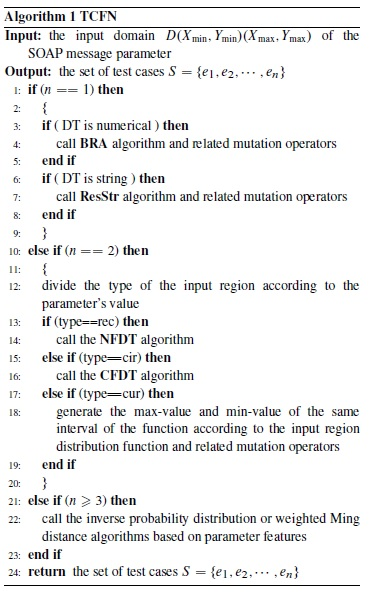
\includegraphics[height=75mm]{Feathergraphics/TCFN.jpg}
%\end{frame}
\begin{frame}{WSVTS framework}
	\centering
	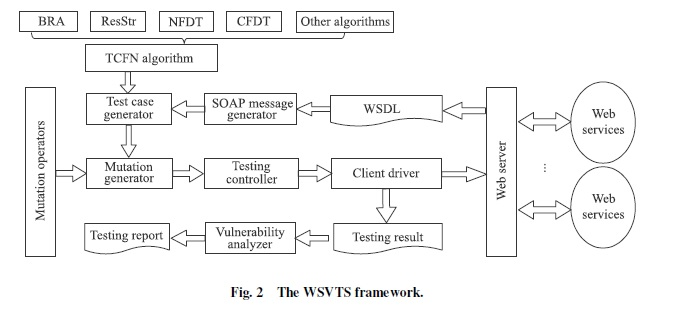
\includegraphics[height=55mm]{Feathergraphics/WSVTS.jpg}
\end{frame}
\begin{frame}{Contd\dots}
	\begin{block}{Flow Chart}
		\centering
		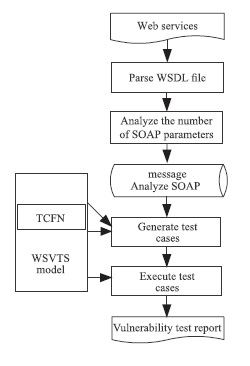
\includegraphics[height=65mm]{Feathergraphics/WSflowChart.jpg}
		
	\end{block}
\end{frame}

\section{Proposed Methods}
{\1
\begin{frame}[plain,noframenumbering]
\begin{block}{}

  \finalpage{\LARGE\textbf{Proposed Methods}}
  \end{block}
\end{frame}}

\begin{frame}{}
	\begin{block}{Propoesed Modification}
		\begin{itemize}
			\item Based on the [9], XPath Injection is an important vulnerability among web service.
			\item The base paper works on data part of web service and is not considering XPath Injection attacks.
			\item The base paper is modified so as to identify Xpath Injection Attacks.
			\item XML structure of the SOAP message is mutated so as to identify the Xpath Injection Attacks.
		\end{itemize}
	\end{block}
	
\end{frame}
%\section{Conclusion}
\begin{frame}{Conclusion}{}
	\begin{block}{}


	\begin{itemize}
		\item Web service Testing is conducted by considering mutation approach.
		\item Xpath Injection attack of web service is tested by considering SOAP message mutation approach.
		
	\end{itemize}
		\end{block}
\end{frame}


\begin{frame}[t,allowframebreaks]
	\frametitle{References}
	\begin{enumerate}
		\item [1] Automated Robustness Testing of Web Service.\\
		Evan Martin, Suranjana Basu, Tao Xie
		\item [2] Exploring Perturbation Based Testing for Web Service \\
		Lourival F de Alemeida and Silvia R Vergilio
		\item [3] Efficient Web Services Message Exchange by SOAP Bundling Framework\\
		Toshiro Takase,Keishi Tajima
		\item [4] Generating Test Cases for Web Services Using Data Perturbation\\
		Jeff Offutt \& Wuzhi Xu
		\item [5] Adaptive Random Testing: the ART of Test Case Diversity\\
		Tsong Yueh Chen , Fei-Ching Kuo, Robert G. Merkel, T.H. Tse
		\item [6] Testing Web Services by XML Perturbation\\
		Wuzhi Xu, Jeff Offutt and Juan Luo

		\item [7] Combinatorial Mutation Approach to Web Service Vulnerability Testing \\
		Qing Li , Jinfu Chen , Yongzhao Zhan, Chengying Mao, Huanhuan Wang
		\item [8] API based Security solutions for
		Communication among Web Services\\
		A. Kanchana Rajaram, B. Chitra Babu, and C. Kishore Kumar R
		\item [9] A New Taxonomy of Web attacks suitable for efficient encoding\\
		Gonzalo Alvarez,Slobodan Petrovic
		%\item [10] Web Service Vulnerabilities
	\end{enumerate}
\end{frame}




%Final Page
{\1
\begin{frame}[plain,noframenumbering]
  \finalpage{\LARGE Thank you !}
\end{frame}}

\end{document}

%\subsection{Detection of SQL/Xpath Injection Vulnerabilities}
\begin{frame}{3. Effective Detection of SQL/XPath Injection Vulnerabilities in Web Services}{Nuno Antunes, Nuno Laranjeiro, Marco Vieira, Henrique Madeira}
	Command Injection Attacks take advantage of improperly coded applications to inject and execute commands specified by the attacker.\\
	Vulnerabilities allowing SQL Injection and XPath injection are particularly relevant in web services
	\\ Techniques used for identification include
	\begin{itemize}
		\item Penetration Testing (Black box testing)
		\item Code Analysis (White box Testing)
	\end{itemize}
\end{frame}




\begin{frame}{Contd\dots}
	\begin{block}{Detecting XPath Injection}
		Based on five steps
		\begin{enumerate}
			\item Instrument the web service to intercept all
			XPath commands executed.
			\item Generate a workload based on the web service operations, parameters, data types, and input domains.
			\item Execute the workload to learn SQL commands and
			XPath queries, issued by the service.
			\item Generate an attack load based on a large set of
			 XPath Injection attacks.
			\item Execute the attack load to detect vulnerabilities by
			comparing XPath commands executed with the valid ones previously learned
		\end{enumerate}
	\end{block}
	
\end{frame}

%\subsection{Web Service Vulnerabilities}
\begin{frame}{[10] Web Service Vulnerabilities}{}
	\begin{block}{Attacks on Web Services}	
		\begin{itemize}
			\item WSDL Enumeration
			\item Exploiting XML Parsers
			\item Exploiting XML Validators
			\item Error Handling
			\item Xpath Injection
		\end{itemize}
	\end{block}
\end{frame}
